\documentclass[conference,a4paper]{IEEEtran}
\usepackage[T1]{fontenc}
\usepackage{graphicx}
\usepackage{amsmath}
\usepackage{booktabs}
\usepackage{array}
\usepackage{url}
\usepackage[hidelinks]{hyperref}
\hypersetup{pdftitle={Reproducible RTL Evaluation of a VHDL 2x2 Mesh Network-on-Chip with Held-Grant Arbitration},pdfauthor={Anjor Giri, Nidhi Kanoujia, Deven Gaikwad},pdfsubject={Accepted-event measurement and FIFO-depth study; FPGA fabric validation; board testing pending}}
\graphicspath{{figures/}}
% Preserve IEEEtran font sizes, column geometry and spacing.
\title{Reproducible RTL Evaluation of a VHDL $2\times 2$ Mesh Network-on-Chip with Held-Grant Arbitration}
\author{\IEEEauthorblockN{Anjor Giri, Nidhi Kanoujia, Deven Gaikwad}
\IEEEauthorblockA{Department of Electronics and Communication Engineering\\
School of Engineering and Technology\\
DES Pune University, Pune, India}}
\begin{document}
\maketitle
\begin{abstract}
A four-router, 32-bit single-flit mesh Network-on-Chip is implemented in VHDL-2008 with input buffering, dimension-order routing, per-output round-robin arbitration and ready/valid backpressure. The reference depth is four; a held grant retains the selected FIFO head during downstream stalls. Fourteen local GHDL 6.0.0 configurations and fourteen independent Vivado 2026.1/XSim configurations passed. They cover coordinate pairs, directed links, FIFO boundaries, arbitration, concurrency, reset accounting and packet integrity. The original GHDL 4.1.0 93-run RTL study at depths two, four and eight delivers all 82,523 accepted benchmark packets. Empty-network two-hop latency is six clock cycles. A registered arbitration bubble limits each output to 0.5 flits per cycle; increasing FIFO depth under saturated hotspot traffic increases accepted backlog and latency without changing that ceiling. The design targets Spartan-7 xc7s15cpga196-2 and Vivado 2026.1. Archived core out-of-context (OOC) synthesis uses 1,086 lookup tables (LUTs) and 147 flip-flops. The routed finite-demo wrapper uses 1,067 LUTs and 236 flip-flops, with Worst Negative Slack (WNS) +4.571 ns at a 10 ns target. Physical board behavior remains unverified; the attempted Standard Delay Format (SDF) timing simulation failed and is deferred. Results are a small-scale implementation study, not a new routing algorithm or an established advantage over a bus.
\end{abstract}
\begin{IEEEkeywords}
Network-on-Chip, VHDL-2008, FPGA, XY routing, ready/valid, round robin, reproducible RTL simulation.
\end{IEEEkeywords}
\section{Introduction and Research Question}
Packet interconnection separates endpoint computation from the communication fabric, a central motivation in the NoC literature \cite{benini2002,dally2001}. A small FPGA-targeted mesh is useful for studying explicit storage, routing, arbitration and flow-control contracts, provided demonstrations and resource claims are supported by actual evidence.

This work asks: how do conditional source generation load, contention and input FIFO depth affect accepted-packet latency, aggregate throughput, source service and occupancy in a verified four-router single-flit mesh? Local exact-device resource and internal timing observations now supplement that question; board timing and physical validation remain separate.

The contributions are (i) an inspectable VHDL hierarchy with explicit full-FIFO, reset and retained-grant contracts; (ii) an accepted-event scoreboard and a reproducible 93-run evaluation with injection-cohort latency followed through drain; and (iii) a measured depth study that distinguishes admitted backlog from an unchanged destination-service ceiling. A local trace application exposes the same evidence. The study evaluates a small concrete implementation rather than proposing new routing theory or claiming universal NoC superiority.

\section{Related Work and Scope}
Benini and De Micheli motivate network-based SoC communication \cite{benini2002}. Dally and Towles describe a substantially different folded-torus example with conventional virtual-channel buffering \cite{dally2001}; its performance is not assigned to this single-flit mesh. Pande et al. frame topology/performance/cost tradeoffs \cite{pande2005}, motivating controlled definitions rather than borrowed numerical results. Dally and Seitz analyze channel dependencies for routing deadlock \cite{dally1987}, distinguishing dependency cycles from stalled sinks and congestion.

The baseline contains no virtual channels, multi-flit wormhole control, adaptive routing, CPU/AI implementation, Zynq processing system or AXI subsystem. CPU~1, memory controller, CPU~2 and AI accelerator are source/sink traffic-model labels. No bus or fixed-priority reference was implemented. These boundaries keep the measured controller and comparisons reproducible.
\section{Topology, Protocol and Microarchitecture}
\subsection{Coordinates and Packet Contract}
Router indices are $X+2Y$: R00=(0,0), R01=(1,0), R10=(0,1), R11=(1,1). $X$ increases east and $Y$ south. Neighbor pairs 0--1, 0--2, 1--3 and 2--3 create eight directed channels, each with 32-bit data, forward valid and reverse ready. Four local interfaces provide independent injection and ejection.

Table~\ref{tab:packet} defines the shared packet package. Bit 31 is a legal-packet marker, not the external handshake signal. DATA type is 00; reserved priority is ignored by round robin. Unsupported marker/type encodings are outside the hardware input contract and trigger simulation assertions; the synthesized baseline does not contain a type-rejection engine. The four-bit packet ID wraps. A bounded testbench uses unique payload values as transaction identities and still compares the complete 32-bit word.
\begin{table}[t]
\caption{Single-flit packet contract (32 bits)}\label{tab:packet}
\centering\begin{tabular}{ll}\toprule
Bits & Field \\\midrule
31 & Marker=1 \\
30:29 & DATA type=00 \\
28:27 & Source X at 28, Y at 27 \\
26:25 & Destination X at 26, Y at 25 \\
24:21 & Four-bit packet ID \\
20:19 & Reserved priority \\
18:0 & 19-bit payload \\\bottomrule
\end{tabular}
\end{table}
\begin{figure*}[t]
\centering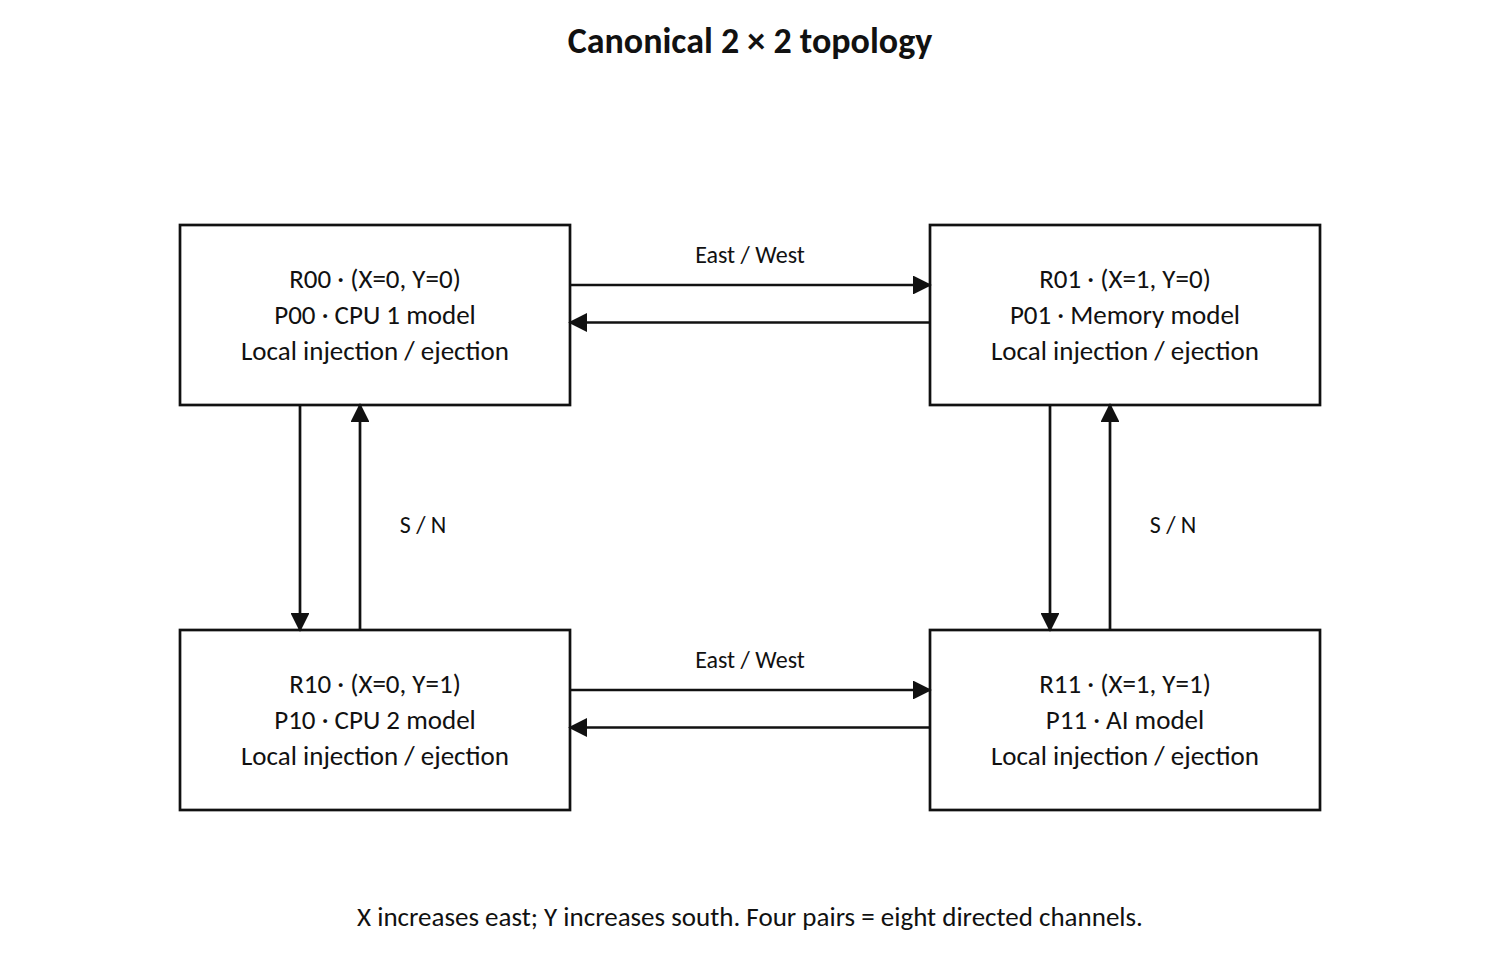
\includegraphics[width=0.91\textwidth]{01_topology.png}
\caption{Canonical orientation and separate directions for each neighbor pair. Endpoint names denote traffic models attached through Local. The drawing is derived from the implemented topology.}\label{fig:topology}
\end{figure*}
\subsection{FIFO and Handshake Behavior}
Acceptance occurs on a rising edge with reset inactive and external valid and ready both one. The producer retains data and valid through a stall and does not wait for ready before asserting valid. Reset is synchronous active-high and overrides normal transfers; producers deassert valid during reset. FIFO occupancy and pointers reset, inaccessible memory need not be cleared, and the testbench records accepted pending packets as explicit reset discards.

Each corner has three active input FIFOs; inactive boundary ports are tied off. Input ready depends only on registered occupancy, excluding a combinational ready loop through the mesh. At nonempty/nonfull occupancy a push and pop may both succeed. An empty FIFO cannot bypass a simultaneous arrival. A full FIFO refuses a push even if a pop occurs at the same edge, allowing retry on the following cycle. Pointer wrap explicitly supports non-power-of-two depth.

Logical packet capacity is $12\times D\times 32$ bits, or 1536 bits at the reference depth 4. This is reserved data capacity, not a synthesized LUT, flip-flop or Block RAM count.
\subsection{Route, Requests and Retained Grant}
The route unit selects East/West if current and destination $X$ differ; otherwise South/North if $Y$ differs; otherwise Local. An arrived packet selects Local before any outgoing link. Thus $0\to3$ takes $0\to1\to3$ and $2\to1$ takes $2\to3\to1$. Legal routes are monotone in each dimension and never turn from $Y$ back to $X$, giving the standard acyclic channel-dependency argument \cite{dally1987}. This model-level reasoning does not establish bounded wall-clock progress when sinks refuse forever, nor exhaustive formal correctness of the RTL.

Each occupied input head requests one output. Each active output has an independent rotating arbiter and a one-hot registered held grant. The crossbar muxes retained FIFO heads. A stalled grant cannot change and its selected FIFO cannot pop. Acceptance pops that FIFO, clears the grant and advances the pointer to one past the winner. No extra output packet register is required. Separate inputs can transfer to nonconflicting outputs simultaneously.

The implemented output controller has FREE and HELD states. A FREE arbiter captures a request at one edge and can transfer at the next. After acceptance there is one arbitration bubble before another grant can transfer. Therefore
\begin{equation}
T_{\mathrm{output}}\leq \frac{1}{2}\quad\text{flits/cycle}.
\end{equation}
A packet entering an empty FIFO at edge $c$ can first leave at $c+2$. With ready sinks and empty intermediate queues, local, one-hop and two-hop exclusive latencies are two, four and six cycles. This contract matches the recorded examples; stalls and contention add delay.
\section{Verification Methodology}
The portable suite, rerun locally with GHDL 6.0.0, contains four FIFO depth runs (1,3,4,8), one route test, one arbiter test, four corner-router tests, one finite-demo test and three directed mesh depth runs. All 14 passed, as did a separate fourteen-configuration Vivado 2026.1/XSim suite. The 93 original controlled benchmarks retain GHDL 4.1.0 provenance. The depth-four mesh baseline passed before the controlled depth comparisons. Module checks cover full/empty, wrap, simultaneous operations, held arbitration through stalls and rotation. Router tests contend three active inputs at every one of the twelve active outputs, then require simultaneous nonconflicting output transfers.

The mesh scoreboard records only accepted injections. For each unique transaction it stores the full packet, injection edge, current location, hop count and per-source/destination stream sequence. Link accepts must follow the expected XY direction. Delivery accepts must match the full word, destination, shortest-hop count, unique pending entry and stream order. Global order between independent sources is not asserted. Assertions also check unknown controls after reset, one-hot grants, one-input selection, boundary use and stall stability. Watchdogs bound runs and drain.

The directed suite covers all 16 coordinate pairs and all 8 directed links, all-four-node congestion, sink stalls, capacity and reset with pending traffic. At depth 4 its actual accounting is
\begin{equation}
106\ \text{accepted}=74\ \text{delivered}+32\ \text{reset discards}.
\end{equation}
No unexplained pending transaction remains. Reset discards are prescribed flush behavior, not the controlled performance benchmark. The arbiter test bounds a persistent requester by five successful grants in the five-input case; stalled wall-clock cycles do not consume that bound.
\begin{figure*}[t]
\centering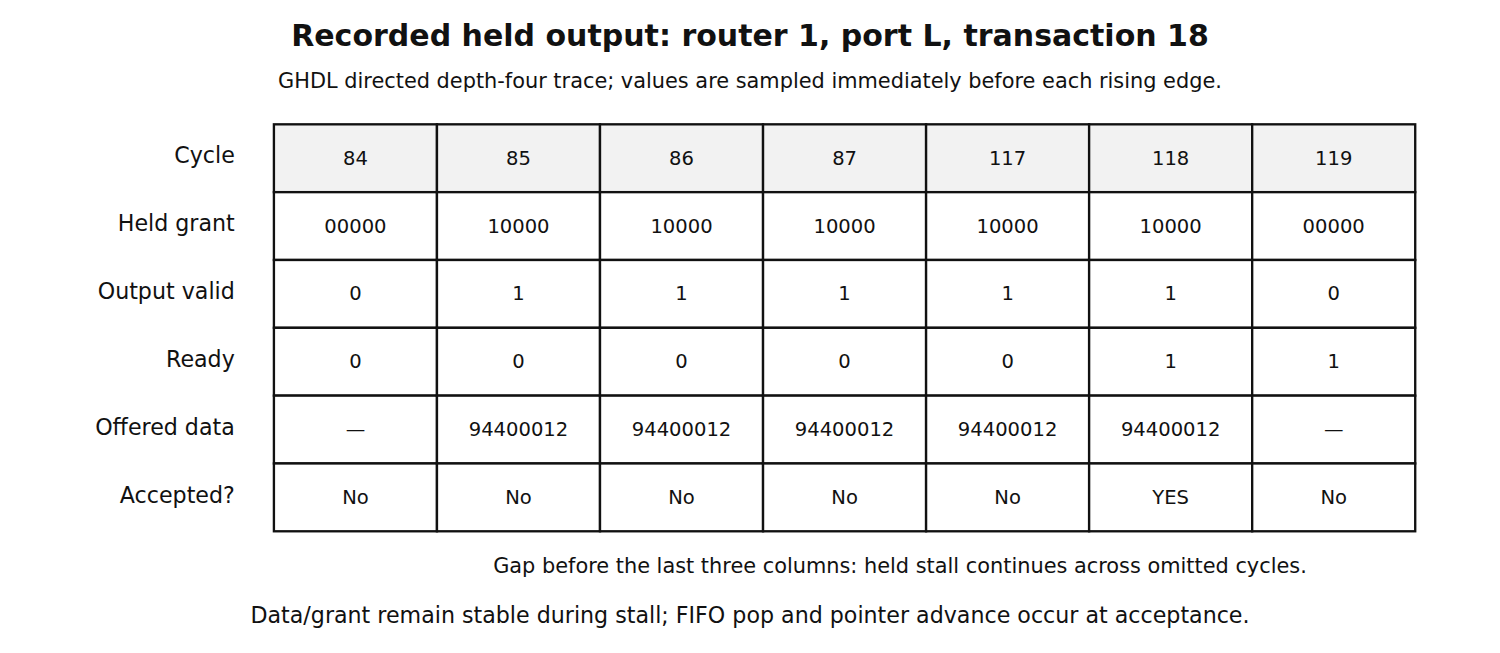
\includegraphics[width=\textwidth]{06_handshake_trace.png}
\caption{Actual CSV-derived pre-edge output state during a held grant. Omitted stalled cycles are labelled. Data/grant retain until acceptance; this is a recorded-state table, not an XSim waveform screenshot.}\label{fig:hold}
\end{figure*}
\section{Controlled Experiments and Metrics}
\subsection{Configurations and Traffic}
There are 93 runs: 3 FIFO depths times 31 configurations. Each depth executes no-load, disjoint, burst and sustained deterministic cases; all-to-all and hotspot each use four gates and three seeds; sink stall uses three seeds. Gates are 0.10,0.25,0.50,0.90; seeds are 101,202,303. Every run has 100 warm-up cycles, 1000 measurement cycles, a drain bound of 5000 cycles and a 30,000-edge watchdog. The simulation clock is 10 ns for event scheduling; no physical oscillator is established.

No-load sends $0\to3$ every 40 cycles. Disjoint sources 0/1 send to 2/3 every four cycles. All-to-all selects destinations from xorshift32 bits, including Local; hotspot destinations are 1. Burst generates in the first 20 of every 100 cycles to $(s+3)\bmod4$. Sustained sources always re-offer to 1 after prior acceptance. Sink-stall traffic uses gate 0.5 to $(s+3)\bmod4$, while sinks refuse during the first 60 of every 160 cycles.

Sources hold one pending request and generate only when free. A configured gate is consequently conditional on source-slot availability, not an independent arrival rate. Repeated stalled valid cycles count offered demand. The PRNG advances for all sources every cycle, including blocked ones. Matched seeds and sink schedules therefore do not ensure an identical accepted transaction population across depths; backpressure affects which random words are used to launch packets.
\subsection{Accepted-Event Definitions}
For accepted injection and delivery edges $c_A(u)$ and $c_D(u)$,
\begin{equation}
L(u)=c_D(u)-c_A(u).
\end{equation}
The reported latency cohort is the set of packets injected during measurement; their drain completions are retained. Mean, median and nearest-rank 95th percentile use this cohort and its sample count $n$. This avoids censoring the slowest accepted packets at the measurement boundary.

Aggregate throughput is
\begin{equation}
T=\frac{N_{D,\mathrm{measurement}}}{1000},
\end{equation}
while accepted load uses injection count and offered demand uses valid presentation count over the same interval. Window accepted and delivered counts may differ due to warm-up/drain boundaries. Whole-run accounting requires accepted=delivered+reset-discarded+outstanding; all controlled runs require the latter two terms zero.

Source service index is
\begin{equation}
J=\frac{(\sum_{i=0}^{3}s_i)^2}{4\sum_{i=0}^{3}s_i^2},
\end{equation}
where $s_i$ counts source $i$ deliveries during measurement. Unequal eligibility makes this descriptive rather than an arbiter proof. FIFO mean/peak use pre-edge samples from twelve active inputs. Stalls are output port-cycles, potentially several per clock cycle. Only flits/cycle and cycle latency are reported; no physical bits/s, power or fMAX is inferred.
\begin{table*}[t]
\caption{Actual depth-four results, seed 101. Latency cohort accepted in measurement, with drain completions. Rates are per 1000-cycle measurement window.}\label{tab:results}
\centering\begin{tabular}{lrrrrrrr}\toprule
Workload & Gate & $n$ & Mean cycles & Median & P95 & Accepted/cycle & Delivered/cycle \\\midrule
No load & 1.00 & 25 & 6.000 & 6 & 6 & 0.025 & 0.025 \\
Disjoint & 1.00 & 500 & 4.000 & 4 & 4 & 0.500 & 0.500 \\
All-to-all & 0.50 & 1619 & 12.035 & 11 & 24 & 1.619 & 1.624 \\
Hotspot & 0.50 & 500 & 53.692 & 46 & 117 & 0.500 & 0.500 \\
Burst & 1.00 & 520 & 8.846 & 9 & 11 & 0.520 & 0.520 \\
Sustained & 1.00 & 499 & 53.749 & 46 & 117 & 0.499 & 0.500 \\
Sink stall & 0.50 & 1249 & 24.601 & 14 & 77 & 1.249 & 1.255 \\
\bottomrule\end{tabular}
\end{table*}
\section{Measured Results and Discussion}
All 93 controlled RTL runs completed with 82,523 accepted packets and 82,523 deliveries, zero reset discards and zero outstanding entries. Under these tests, no unexplained loss, duplicate, misroute or stream reorder was observed. Source and trace SHA-256 values are included with configuration, raw CSV and actual logs. The measurement runner invokes GHDL; JavaScript performs trace analysis rather than behavioral router simulation.

Table~\ref{tab:results} gives selected depth-four seed 101 configurations. The no-load two-hop cohort contains 25 packets, each with six-cycle latency. Independent outputs permit aggregate throughput above 0.5: all-to-all gate 0.90 at this depth/seed achieves 1.656 flits/cycle. This is a workload-specific observation, not a universal bandwidth claim.

Fig.~\ref{fig:alltoall} compares all-to-all run means across three seeds. Increasing accepted load raises queueing latency. Deeper FIFOs can alter accepted load and population under congestion; those differences preclude attributing every change to a fixed-arrival latency effect.
\begin{figure*}[t]
\centering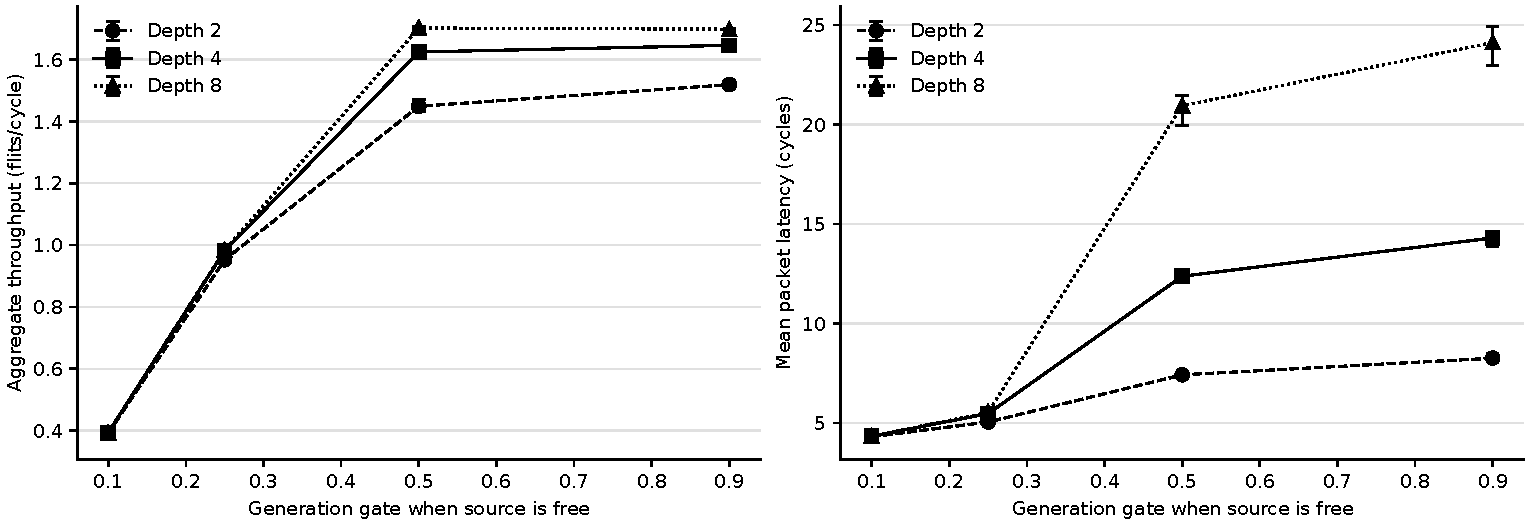
\includegraphics[width=\textwidth]{13_all_to_all_results.pdf}
\caption{All-to-all arithmetic mean of three run metrics. Whiskers show observed minimum/maximum across seeds, not statistical confidence intervals. Generation gate is conditional on a free source slot.}\label{fig:alltoall}
\end{figure*}

The saturated-destination ablation in Table~\ref{tab:depth} retains the same controller. Throughput is 0.5 at every depth, matching the bubble ceiling. Mean latency grows as larger queues admit more pending work. Additional buffering does not remove the output service bottleneck.
\begin{table*}[t]
\caption{Deterministic sustained hotspot depth comparison. Logical capacity is not FPGA utilization.}\label{tab:depth}
\centering\begin{tabular}{rrrrrr}\toprule
Depth & Logical packet bits & Cohort $n$ & Mean cycles & P95 cycles & Flits/cycle \\\midrule
2 & 768 & 499 & 26.090 & 57 & 0.500 \\
4 & 1536 & 499 & 53.749 & 117 & 0.500 \\
8 & 3072 & 499 & 108.251 & 237 & 0.500 \\
\bottomrule\end{tabular}
\end{table*}

Source Jain service is approximately 0.90 under the documented sustained hotspot. Rotating priority divides successful grants among inputs, not original global sources. Sources 2/3 share the R11-to-R01 merge, while 0 and 1 occupy separate R01 input streams. This end-to-end imbalance is consistent with the tested local successful-grant fairness bound. No-load/disjoint source indices are also affected by the number of eligible sources.
\section{FPGA Implementation Evidence and Limits}
The exact part is xc7s15cpga196-2. Local Vivado 2026.1, SW Build 6511674, executed XSim, core synthesis and fabric-only demonstration routing. Tool and constraint meanings follow AMD guidance \cite{ug900,ug901,ug903,ug906}. Device/package documents do not establish board pins \cite{ug475,ds189}. Out-of-context (OOC) implementation evaluates internal fabric without a complete board interface.

Table~\ref{tab:fpga} separates three observations at DEPTH=4 and a 10 ns clock target. The archived core synthesis and later GUI core screenshots differ by one LUT and by pre-route timing. They are separate records, not a measured optimization. The routed demo adds four finite source/sink models; its cost cannot replace core cost. The exposed GUI core requires 1,774 logical I/O signals against 100 package pins, so it is not a usable board top. OOC I/O=0 does not imply pin-free hardware.
\begin{table*}[t]
\caption{Separate Vivado 2026.1 observations for xc7s15cpga196-2, DEPTH=4, 10 ns target.}
\label{tab:fpga}\centering
\begin{tabular}{llrrrr}\toprule
Source and stage & Top & LUT & FF & WNS (ns) & TNS (ns) \\\midrule
Archived OOC synthesis & noc\_2x2\_core & 1086 & 147 & +6.233 & 0 \\
Later GUI synthesis, pre-route & noc\_2x2\_core & 1085 & 147 & +6.129 & 0 \\
Archived OOC routing & noc\_fpga\_demo\_top & 1067 & 236 & +4.571 & 0 \\\bottomrule
\end{tabular}
\end{table*}

The routed demo uses 841 logic LUTs and 226 LUTs as memory, with zero BRAM or DSP. All 1,468 routable nets are fully routed, with zero routing errors. Of 1,845 logical nets, 377 require no routing; logical-net and routable-net totals are different populations. Routed WHS is +0.066 ns, THS 0, WPWS +3.870 ns and TPWS 0. Positive WNS is a setup margin on analyzed paths; TNS=0 means no negative setup slack in that analyzed set. Internal static timing is not a packet-latency measurement or maximum-frequency measurement.

clock\_only.xdc establishes the design target. The later GUI core has 137 missing-input-delay and 648 missing-output-delay findings. No external delays, pins, I/O standards or blanket false paths are fabricated. Routed DRC retains CFGBVS-1 (unspecified configuration-bank voltage) and RTSTAT-10 (unloaded nets). These limits prevent complete board signoff despite passing internal timing.

The original XSim waveform in Fig.~\ref{fig:xsim} shows receiver presentation before a Local delivery. Packet 0x80200001 is accepted at 25 ns and delivered at 45 ns, two cycles. The depth-four test ends at 2400 ns with the documented 106/74/32 reset accounting. A separate post-route functional console extract reports \texttt{PASS tb\_demo\_postroute 64 delivered} at 530 ns. This supplemental extract was supplied after the Oct-4 archive; its generated netlist, SDF and checkpoint bytes were not attached.

The attempted Verilog timing netlist with an adapted VHDL testbench achieved successful SDF annotation, then reported \texttt{Demo status/count failure} at 20150 ns. It remains unresolved/deferred; process exit code zero is not a functional PASS. UG900 supports timing netlists in Verilog and functional VHDL netlists without SDF \cite{ug900}. Functional netlist success and positive static timing do not resolve the failed timing simulation. No physical board, bitstream or power measurement is supplied.
\begin{figure*}[t]
\centering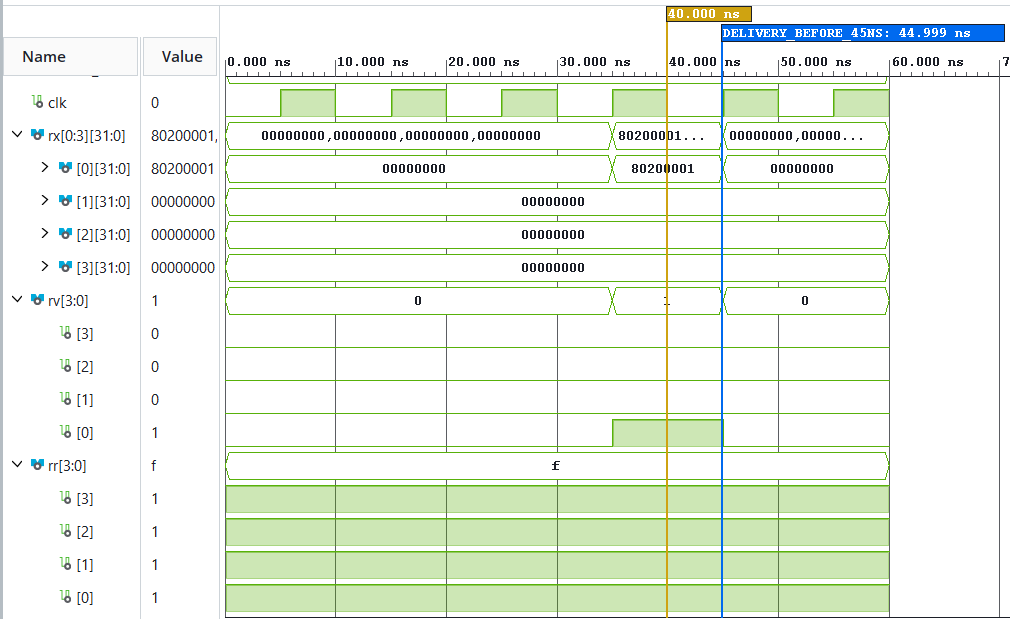
\includegraphics[width=0.69\textwidth]{xsim_delivery_crop.png}
\caption{Original Screenshot 10, cropped to receiver signals in XSim tb\_noc\_2x2. The yellow value cursor is 40 ns; the blue marker is 44.999 ns, before the delivery rising edge at 45 ns. RX(0)=0x80200001 and RV(0)=RR(0)=1 indicate presentation for Local delivery. This is not an inter-router or physical-board transfer.}\label{fig:xsim}
\end{figure*}
\begin{figure*}[t]
\centering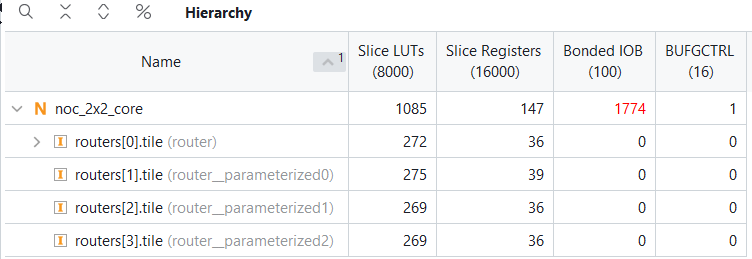
\includegraphics[width=0.74\textwidth]{core_gui_utilization_crop.png}
\caption{Original Screenshot 16, cropped to the later GUI synthesis hierarchy. The core has 1,085 LUTs and 147 registers. These are distinct from the archived OOC core's 1,086 LUTs. I/O overuse is visible; the exposed core is not the board top.}\label{fig:coregui}
\end{figure*}
\begin{figure*}[t]
\centering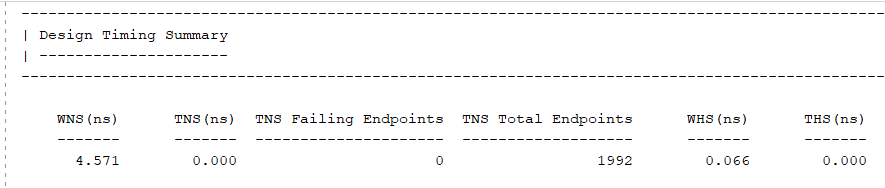
\includegraphics[width=0.82\textwidth]{demo_routed_timing_crop.png}
\caption{Original Screenshot 27, cropped to the routed demo setup/hold summary. WNS +4.571 ns, TNS 0, WHS +0.066 ns and THS 0 cover internally constrained paths. The 10 ns target and missing external timing remain separate from physical-board signoff.}\label{fig:routed}
\end{figure*}
\section{Reproducibility and Threats to Validity}
The delivered source includes packet package, eleven design files, six testbenches, compile order, Windows scripts, 93 raw trace/log pairs, metrics/configuration/hashes, corrected SVG figures and a local TypeScript application. The dashboard steps exact recorded edges, validates schemas and completion identity, and distinguishes bundled RTL evidence from user-supplied provenance. Incomplete measurement-state coverage produces unavailable rates. Resource imports now contain the archived core and routed-demo report summaries, with run scopes retained. It has no physical live feed or Python backend.
\begin{figure*}[t]
\centering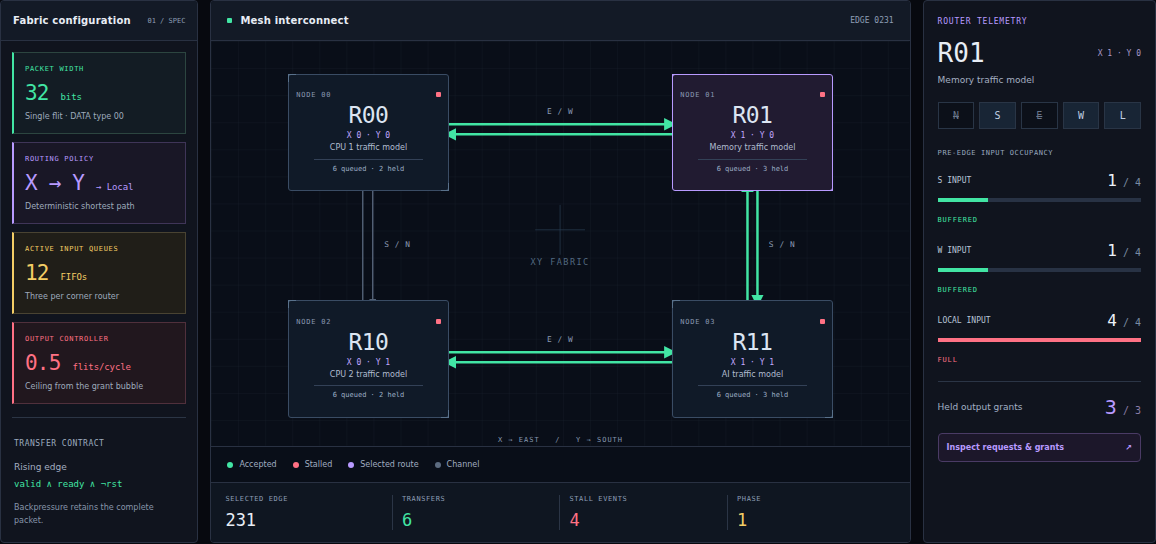
\includegraphics[width=\textwidth]{15_dashboard_capture.png}
\caption{Recorded-trace application at directed-d4 edge 231: six accepted link transfers, four stall events and full R01 Local input. Eight directional channels are displayed separately. This screenshot shows software replay of GHDL evidence, not physical live FPGA telemetry.}\label{fig:dashboard}
\end{figure*}

Assertion-driven simulation is finite testing, not exhaustive formal verification. Four routers, synthetic traffic and model endpoints limit external validity. Shared input queues cause head-of-line blocking. Three seeds and 1000 cycles offer limited statistical coverage and do not prove steady state. Closed-loop generation and accepted-population differences complicate saturated depth comparisons. No equally conditioned bus/fixed-priority reference was executed. Exact-part fabric resource and internal timing observations are available, but external interface timing, physical behavior and power remain unverified. The SDF timing simulation failed. Finite tests, generic synthesis and frontend checks cannot replace those remaining gates.
\section{Conclusion and Future Work}
A reproducible VHDL single-flit mesh and accepted-event measurement workflow were created and verified with fourteen portable tests, fourteen independent XSim configurations and the original 93 GHDL 4.1.0 RTL experiments. The measured controller has a six-cycle empty two-hop path and a 0.5-flit/cycle per-output ceiling. Saturated depth changes expose a backlog/latency tradeoff rather than improved destination service. These conclusions are bounded by the recorded workloads and tool evidence.

Local XSim, core synthesis and demo OOC routing are complete. Routed internal WNS is +4.571 ns at 10 ns, with TNS 0; these results do not establish board timing. The supplemental functional console reports 64 deliveries, while SDF timing remains failed/deferred. Verified board data and resolved simulation limits are required before stronger hardware claims. Future studies may examine a bubble-free arbiter, separated queues/virtual channels, longer trials and an equally conditioned reference interconnect. Those features and comparisons are not implemented claims in this manuscript.
\section*{Acknowledgment}
The project team acknowledges Dr. Madan Mali, faculty and mentor, and the Department of Electronics and Communication Engineering, School of Engineering and Technology, DES Pune University.

OpenAI ChatGPT/Codex assisted with VHDL/TypeScript code preparation, automated analysis, diagrams and manuscript drafting. Benchmark measurements were obtained by executing the supplied RTL in GHDL 4.1.0. Additional local checks used GHDL 6.0.0 and Vivado 2026.1; supplemental netlist results are supplied console evidence. Human author review and approval are required before submission.
\bibliographystyle{IEEEtran}
\bibliography{references}
\end{document}
